%  LaTeX support: latex@mdpi.com 
%  For support, please attach all files needed for compiling as well as the log file, and specify your operating system, LaTeX version, and LaTeX editor.

% see also Google doc at https://docs.google.com/document/d/1Hitne_x4s-Iivetij_XnJBoShJj95FDxYIDc6PRfBDQ/edit#heading=h.2usqgv7yajxv
%=================================================================
\documentclass[remotesensing,article,submit,pdftex,moreauthors]{Definitions/mdpi} 
% For posting an early version of this manuscript as a preprint, you may use "preprints" as the journal and change "submit" to "accept". The document class line would be, e.g., \documentclass[preprints,article,accept,moreauthors,pdftex]{mdpi}. This is especially recommended for submission to arXiv, where line numbers should be removed before posting. For preprints.org, the editorial staff will make this change immediately prior to posting.

%--------------------
% Class Options:
%--------------------
%----------
% journal
%----------
% Choose between the following MDPI journals:
% acoustics, actuators, addictions, admsci, adolescents, aerospace, agriculture, agriengineering, agronomy, ai, algorithms, allergies, alloys, analytica, animals, antibiotics, antibodies, antioxidants, applbiosci, appliedchem, appliedmath, applmech, applmicrobiol, applnano, applsci, aquacj, architecture, arts, asc, asi, astronomy, atmosphere, atoms, audiolres, automation, axioms, bacteria, batteries, bdcc, behavsci, beverages, biochem, bioengineering, biologics, biology, biomass, biomechanics, biomed, biomedicines, biomedinformatics, biomimetics, biomolecules, biophysica, biosensors, biotech, birds, bloods, blsf, brainsci, breath, buildings, businesses, cancers, carbon, cardiogenetics, catalysts, cells, ceramics, challenges, chemengineering, chemistry, chemosensors, chemproc, children, chips, cimb, civileng, cleantechnol, climate, clinpract, clockssleep, cmd, coasts, coatings, colloids, colorants, commodities, compounds, computation, computers, condensedmatter, conservation, constrmater, cosmetics, covid, crops, cryptography, crystals, csmf, ctn, curroncol, currophthalmol, cyber, dairy, data, dentistry, dermato, dermatopathology, designs, diabetology, diagnostics, dietetics, digital, disabilities, diseases, diversity, dna, drones, dynamics, earth, ebj, ecologies, econometrics, economies, education, ejihpe, electricity, electrochem, electronicmat, electronics, encyclopedia, endocrines, energies, eng, engproc, ent, entomology, entropy, environments, environsciproc, epidemiologia, epigenomes, est, fermentation, fibers, fintech, fire, fishes, fluids, foods, forecasting, forensicsci, forests, foundations, fractalfract, fuels, futureinternet, futureparasites, futurepharmacol, futurephys, futuretransp, galaxies, games, gases, gastroent, gastrointestdisord, gels, genealogy, genes, geographies, geohazards, geomatics, geosciences, geotechnics, geriatrics, hazardousmatters, healthcare, hearts, hemato, heritage, highthroughput, histories, horticulturae, humanities, humans, hydrobiology, hydrogen, hydrology, hygiene, idr, ijerph, ijfs, ijgi, ijms, ijns, ijtm, ijtpp, immuno, informatics, information, infrastructures, inorganics, insects, instruments, inventions, iot, j, jal, jcdd, jcm, jcp, jcs, jdb, jeta, jfb, jfmk, jimaging, jintelligence, jlpea, jmmp, jmp, jmse, jne, jnt, jof, joitmc, jor, journalmedia, jox, jpm, jrfm, jsan, jtaer, jzbg, kidney, kidneydial, knowledge, land, languages, laws, life, liquids, literature, livers, logics, logistics, lubricants, lymphatics, machines, macromol, magnetism, magnetochemistry, make, marinedrugs, materials, materproc, mathematics, mca, measurements, medicina, medicines, medsci, membranes, merits, metabolites, metals, meteorology, methane, metrology, micro, microarrays, microbiolres, micromachines, microorganisms, microplastics, minerals, mining, modelling, molbank, molecules, mps, msf, mti, muscles, nanoenergyadv, nanomanufacturing, nanomaterials, ncrna, network, neuroglia, neurolint, neurosci, nitrogen, notspecified, nri, nursrep, nutraceuticals, nutrients, obesities, oceans, ohbm, onco, oncopathology, optics, oral, organics, organoids, osteology, oxygen, parasites, parasitologia, particles, pathogens, pathophysiology, pediatrrep, pharmaceuticals, pharmaceutics, pharmacoepidemiology, pharmacy, philosophies, photochem, photonics, phycology, physchem, physics, physiologia, plants, plasma, pollutants, polymers, polysaccharides, poultry, powders, preprints, proceedings, processes, prosthesis, proteomes, psf, psych, psychiatryint, psychoactives, publications, quantumrep, quaternary, qubs, radiation, reactions, recycling, regeneration, religions, remotesensing, reports, reprodmed, resources, rheumato, risks, robotics, ruminants, safety, sci, scipharm, seeds, sensors, separations, sexes, signals, sinusitis, skins, smartcities, sna, societies, socsci, software, soilsystems, solar, solids, sports, standards, stats, stresses, surfaces, surgeries, suschem, sustainability, symmetry, synbio, systems, taxonomy, technologies, telecom, test, textiles, thalassrep, thermo, tomography, tourismhosp, toxics, toxins, transplantology, transportation, traumacare, traumas, tropicalmed, universe, urbansci, uro, vaccines, vehicles, venereology, vetsci, vibration, viruses, vision, waste, water, wem, wevj, wind, women, world, youth, zoonoticdis 
\usepackage{pythonhighlight}
\usepackage{tcolorbox}

%---------
% article
%---------
% The default type of manuscript is "article", but can be replaced by: 
% abstract, addendum, article, book, bookreview, briefreport, casereport, comment, commentary, communication, conferenceproceedings, correction, conferencereport, entry, expressionofconcern, extendedabstract, datadescriptor, editorial, essay, erratum, hypothesis, interestingimage, obituary, opinion, projectreport, reply, retraction, review, perspective, protocol, shortnote, studyprotocol, systematicreview, supfile, technicalnote, viewpoint, guidelines, registeredreport, tutorial
% supfile = supplementary materials

%----------
% submit
%----------
% The class option "submit" will be changed to "accept" by the Editorial Office when the paper is accepted. This will only make changes to the frontpage (e.g., the logo of the journal will get visible), the headings, and the copyright information. Also, line numbering will be removed. Journal info and pagination for accepted papers will also be assigned by the Editorial Office.

%------------------
% moreauthors
%------------------
% If there is only one author the class option oneauthor should be used. Otherwise use the class option moreauthors.

%---------
% pdftex
%---------
% The option pdftex is for use with pdfLaTeX. If eps figures are used, remove the option pdftex and use LaTeX and dvi2pdf.

%=================================================================
% MDPI internal commands
\firstpage{1} 
\makeatletter 
\setcounter{page}{\@firstpage} 
\makeatother
\pubvolume{1}
\issuenum{1}
\articlenumber{0}
\pubyear{2022}
\copyrightyear{2022}
%\externaleditor{Academic Editor: Firstname Lastname}
\datereceived{} 
%\daterevised{} % Only for the journal Acoustics
\dateaccepted{} 
\datepublished{} 
%\datecorrected{} % Corrected papers include a "Corrected: XXX" date in the original paper.
%\dateretracted{} % Corrected papers include a "Retracted: XXX" date in the original paper.
\hreflink{https://doi.org/} % If needed use \linebreak
%\doinum{}
%------------------------------------------------------------------
% The following line should be uncommented if the LaTeX file is uploaded to arXiv.org
%\pdfoutput=1

%=================================================================
% Add packages and commands here. The following packages are loaded in our class file: fontenc, inputenc, calc, indentfirst, fancyhdr, graphicx, epstopdf, lastpage, ifthen, lineno, float, amsmath, setspace, enumitem, mathpazo, booktabs, titlesec, etoolbox, tabto, xcolor, soul, multirow, microtype, tikz, totcount, changepage, attrib, upgreek, cleveref, amsthm, hyphenat, natbib, hyperref, footmisc, url, geometry, newfloat, caption

%=================================================================
%% Please use the following mathematics environments: Theorem, Lemma, Corollary, Proposition, Characterization, Property, Problem, Example, ExamplesandDefinitions, Hypothesis, Remark, Definition, Notation, Assumption
%% For proofs, please use the proof environment (the amsthm package is loaded by the MDPI class).

%=================================================================
% Full title of the paper (Capitalized)
\Title{A new open-source wind lidar ontology}

% MDPI internal command: Title for citation in the left column
\TitleCitation{A new open-source wind lidar ontology}

% Author Orchid ID: enter ID or remove command
\newcommand{\orcidauthorA}{0000-0000-0000-000X} % Add \orcidA{} behind the author's name
%\newcommand{\orcidauthorB}{0000-0000-0000-000X} % Add \orcidB{} behind the author's name
\newcommand{\orcidauthorC}{0000-0001-7221-9800} % Add \orcidC{} behind the author's name

% Authors, for the paper (add full first names)
\Author{Francisco Costa $^{1,\dagger}$\orcidA{}*,
Dexing Liu $^{2}$,
Aidan Keane $^{3}$\orcidC{},
Ashim Giyanani $^{4}$,
Carlo Alberto Ratti $^{5}$
and Andrew Clifton$^{6}$}

%\longauthorlist{yes}

% MDPI internal command: Authors, for metadata in PDF
\AuthorNames{Francisco Costa, Dexing Liu, Aidan Keane, Ashim Giyanani, CarloAlberto Ratti and Andrew Clifton}

% MDPI internal command: Authors, for citation in the left column
\AuthorCitation{Costa, F.; Liu, D.; Keane, A; Giyanani, A; Ratti, C; Clifton, A.}
% If this is a Chicago style journal: Lastname, Firstname, Firstname Lastname, and Firstname Lastname.

% Affiliations / Addresses (Add [1] after \address if there is only one affiliation.)
\address{%
$^{1}$ \quad University of Stuttgart, Allmandring 5b, 70569 Stuttgart ; costa@ifb.uni-stuttgart.de\\
$^{2}$ \quad University of Stuttgart, Allmandring 5b, 70569 Stuttgart ; liu@ifb.uni-stuttgart.de\\
$^{3}$ \quad Wood Renewables, Floor 2 St Vincent Plaza, 319 St Vincent Street, Glasgow, G2 5LP; aidan.keane@woodplc.com\\
$^{4}$ \quad Affiliation 4; e-mail@e-mail.com\\
$^{5}$ \quad Affiliation 5; e-mail@e-mail.com\\
$^{6}$ \quad Affiliation 6; e-mail@e-mail.com}

% Contact information of the corresponding author
\corres{Correspondence: costa@ifb.uni-stuttgart.de; Tel.: +49 711 685 68336}

% Current address and/or shared authorship
\firstnote{Current address: Affiliation 1b.} 
%\secondnote{These authors contributed equally to this work.}
% The commands \thirdnote{} till \eighthnote{} are available for further notes

%\simplesumm{} % Simple summary

%\conference{} % An extended version of a conference paper

% Abstract (Do not insert blank lines, i.e. \\) 
\abstract{
This article reports on an open-source ontology which has been developed with the aim of establishing an industry-wide consensus on wind lidar concepts and terminology.
The article provides an introduction to the wind lidar ontology and gives an overview of its development, and a summary of the aims and achievements.
The ontology serves both reference and educational purposes for wind energy applications and lidar technology.
The article provides an overview of the creation process, the outcomes of the project and the proposed uses of the ontology.
Examples applications are given.
Issues and challenges with writing the ontology are discussed.
}

% Keywords
\keyword{Wind Energy; Lidar; Wind Velocity Measurement; Ontology; Open-Source} 

% The fields PACS, MSC, and JEL may be left empty or commented out if not applicable
%\PACS{J0101}
%\MSC{}
%\JEL{}

%%%%%%%%%%%%%%%%%%%%%%%%%%%%%%%%%%%%%%%%%%
% Only for the journal Diversity
%\LSID{\url{http://}}

%%%%%%%%%%%%%%%%%%%%%%%%%%%%%%%%%%%%%%%%%%
% Only for the journal Applied Sciences
%\featuredapplication{Authors are encouraged to provide a concise description of the specific application or a potential application of the work. This section is not mandatory.}
%%%%%%%%%%%%%%%%%%%%%%%%%%%%%%%%%%%%%%%%%%

%%%%%%%%%%%%%%%%%%%%%%%%%%%%%%%%%%%%%%%%%%
% Only for the journal Data
%\dataset{DOI number or link to the deposited data set if the data set is published separately. If the data set shall be published as a supplement to this paper, this field will be filled by the journal editors. In this case, please submit the data set as a supplement.}
%\datasetlicense{License under which the data set is made available (CC0, CC-BY, CC-BY-SA, CC-BY-NC, etc.)}

%%%%%%%%%%%%%%%%%%%%%%%%%%%%%%%%%%%%%%%%%%
% Only for the journal Toxins
%\keycontribution{The breakthroughs or highlights of the manuscript. Authors can write one or two sentences to describe the most important part of the paper.}

%%%%%%%%%%%%%%%%%%%%%%%%%%%%%%%%%%%%%%%%%%
% Only for the journal Encyclopedia
%\encyclopediadef{For entry manuscripts only: please provide a brief overview of the entry title instead of an abstract.}

%%%%%%%%%%%%%%%%%%%%%%%%%%%%%%%%%%%%%%%%%%
% Only for the journal Advances in Respiratory Medicine
%\addhighlights{yes}
%\renewcommand{\addhighlights}{%

%\noindent This is an obligatory section in “Advances in Respiratory Medicine”, whose goal is to increase the discoverability and readability of the article via search engines and other scholars. Highlights should not be a copy of the abstract, but a simple text allowing the reader to quickly and simplified find out what the article is about and what can be cited from it. Each of these parts should be devoted up to 2~bullet points.\vspace{3pt}\\
%\textbf{What are the main findings?}
% \begin{itemize}[labelsep=2.5mm,topsep=-3pt]
% \item First bullet.
% \item Second bullet.
% \end{itemize}\vspace{3pt}
%\textbf{What is the implication of the main finding?}
% \begin{itemize}[labelsep=2.5mm,topsep=-3pt]
% \item First bullet.
% \item Second bullet.
% \end{itemize}
%}

%%%%%%%%%%%%%%%%%%%%%%%%%%%%%%%%%%%%%%%%%%
\begin{document}

%%%%%%%%%%%%%%%%%%%%%%%%%%%%%%%%%%%%%%%%%%
%\setcounter{section}{-1} %% Remove this when starting to work on the template.
%\section{How to Use this Template}

%The template details the sections that can be used in a manuscript. Note that the order and names of article sections may differ from the requirements of the journal (e.g., the positioning of the Materials and Methods section). Please check the instructions on the authors' page of the journal to verify the correct order and names. For any questions, please contact the editorial office of the journal or support@mdpi.com. For LaTeX-related questions please contact latex@mdpi.com.%\endnote{This is an endnote.} % To use endnotes, please un-comment \printendnotes below (before References). Only journal Laws uses \footnote.

% The order of the section titles is different for some journals. Please refer to the "Instructions for Authors” on the journal homepage.

\section{Introduction}
Many aspects of wind energy resource assessment and inflow characterization require accurate measurement of wind speed, wind direction and turbulence. In recent years, measurement of wind speeds with lasers, based upon the lidar (Light Detection And Ranging) system, has provided a modern alternative to the traditional meteorological mast. Wind lidar makes use of the principle of optical Doppler shift between the reference radiation and radiation backscattered by aerosol particles to measure radial wind velocities at distances up to several kilometers \cite{ref-Liu}.
Within the field of wind energy, there has been a general move towards adoption of lidar as a cost effective, self-contained and adaptable solution to wind resource measurement.
The use of wind lidars is now widely accepted within the wind energy sector and there has been an associated increase in the technological development of lidar devices and in use cases, and incorporation within a number of IEC standards \cite{ref-IEC61400-12-1, ref-IEC61400-50-3}.

The interest in wind lidar has led to it becoming a research field in its own right, and as a result there has been a multitude of technical advancements and a corresponding plethora of lidar specific concepts and terminology. 
Further, lidar manufacturers use a variety of different concept definitions, conventions and data formats.
As a result, there exist many difficulties and challenges in communication and lidar knowledge transfer, which may be the case in particular for early stage researchers and engineers. This situation has given rise to the need for a system to ensure consistency and comprehension within the field.

To address these issues, academia and industry have been working towards consensus and standardization, and several examples are notable:
The global initiative project e-WindLidar focused on development of wind lidar community based tools and data standards, and published a lidar data form to make them Findable, Accessible, Interoperable and Reusable (FAIR) \cite{ref-Vasiljevi}; 
The IEA Task 52 (previously Task 32) brings together researchers and industry stakeholders to collaborate on the standardization, research and development, and knowledge exchange of wind lidar \cite{ref-Clifton-Schlipf};
The OpenLidar project coordinated by the Stuttgart Wind Energy developed a architecture of an open-source remote wind sensing lidar that can be used for teaching, research, and product development \cite{ref-SWE}.

While these initiatives have been successful, further effort is required to capitalise on their achievements and bring further consensus and standardization within a growing lidar community.
In recognition of this, an open-source ontology has been developed with the aim of establishing an industry-wide consensus on wind lidar concepts and terminology.
An ontology defines a common vocabulary within a domain, providing a means to share information in the domain, and includes machine-interpretable definitions of fundamental concepts and the relations among them.
Many disciplines now develop standardised ontologies that domain experts can use to share and annotate information in their fields \cite{ref-Noy}.
An ontology serves several purposes: sharing the common understanding of the structure of information; making the domain assumptions explicit; and, enabling reuse and analysis of the domain knowledge.

The wind lidar ontology \cite{ref-Clifton-Costa} was created as a subtask of the IEA Task 32, and has been taken on by a group of academics and industry engineers.
This has resulted in the online publication of the latest version of wind lidar ontology \cite{ref-OntoWeb}.
The wind lidar ontology provides an introduction to the fundamental concepts and terminology relating to lidar hardware and software, lidar installation and measurement, data generation, processing, and analysis.
The ontology provides guidelines for a common conceptual architecture for lidar design, modelling and analysis.
The ontology includes the lidar module design according to the OpenLidar Architecture, atmospheric parameters, data configuration and measurement principles.
It is hoped that the ontology will play a part in the development of an industry-wide consensus on lidar concepts, and the standardization of lidar terminology.
The ontology is well placed to facilitate reuse of the domain knowledge and collaboration amongst researchers and engineers.

The lidar ontology scope includes wind energy applications and lidar technology.
The lidar ontology has been developed as an open-source code repository, with the purpose of allowing
free access to users, with options to contribute and redistribute content.
The lidar ontology serves several purposes: A reference source and dictionary for users, and will be of particular
use for new entrants to the field of wind energy;
A variable definition reference for datasets for original equipment manufacturers (OEMs) delivering data to clients;
An input resource for wind modelling and lidar simulations.
As an open-source code repository, the lidar ontology will be subject to ongoing development, with individual releases identified with release version numbers.
The definitions are available to be downloaded from the code repository.

This article provides an introduction to the wind lidar ontology, and gives an overview of its structure and development. Section \ref{sec:Methodology} provides an overview of the ontology methodology. The results are presented in Section \ref{sec:Results} and are discussed in Section \ref{sec:Discussion}. The general outlook for the program is presented in Section \ref{sec:Outlook}.


\section{Methodology}
\label{sec:Methodology}
A controlled vocabulary is a carefully selected list of words and phrases within a specific domain of knowledge, which are used to tag units of information so that they may be retrieved by a search.
Metadata may be specified in accordance with a controlled vocabulary, providing clear and concise representation of data sets, and allowing data to be structured, stored, maintained and shared in a consistent manner. 
Each item within the controlled vocabulary may be regarded as a concept
within the specific domain of knowledge.

The Resource Description Framework (RDF) is a standard model for data interchange on the Web \cite{ref-W3C-RDF}.
RDF is commonly used to model a controlled vocabulary and define properties, relationships, constraints and axioms among its concepts.
RDF, therefore offers the opportunity to digitise, express and handle knowledge organisation systems in a machine-readable format.
The Simple Knowledge Organisation System (SKOS) \cite{ref-W3C-SKOS} offers standards to create data models for metadata, and jointly with RDF facilitates the provision of standardise data organisation models to server machines.

\subsection{Taxonomy and ontology}
A taxonomy is a type of controlled vocabulary in which concepts are related in a hierarchical order or sorted into categories.
An ontology is a type of controlled vocabulary
which identifies and distinguishes concepts and their relationships.

The first step in building a {\it lidar taxonomy} is to create a list of terms, or concepts, related to the wind lidar knowledge domain. To do so, the authors followed the ``Expert elicitation" approach to establish a consensus position. In this approach, experts in the relevant topics gathered in a collaborative way to define the hierarchy of terms and concepts. Figure \ref{fig:tax} illustrates the highest levels of the lidar taxonomy, from the broadest term ``wind lidar" to the narrower terms \cite{ref-IRPWind}.
\begin{figure}[h]
    \centering
    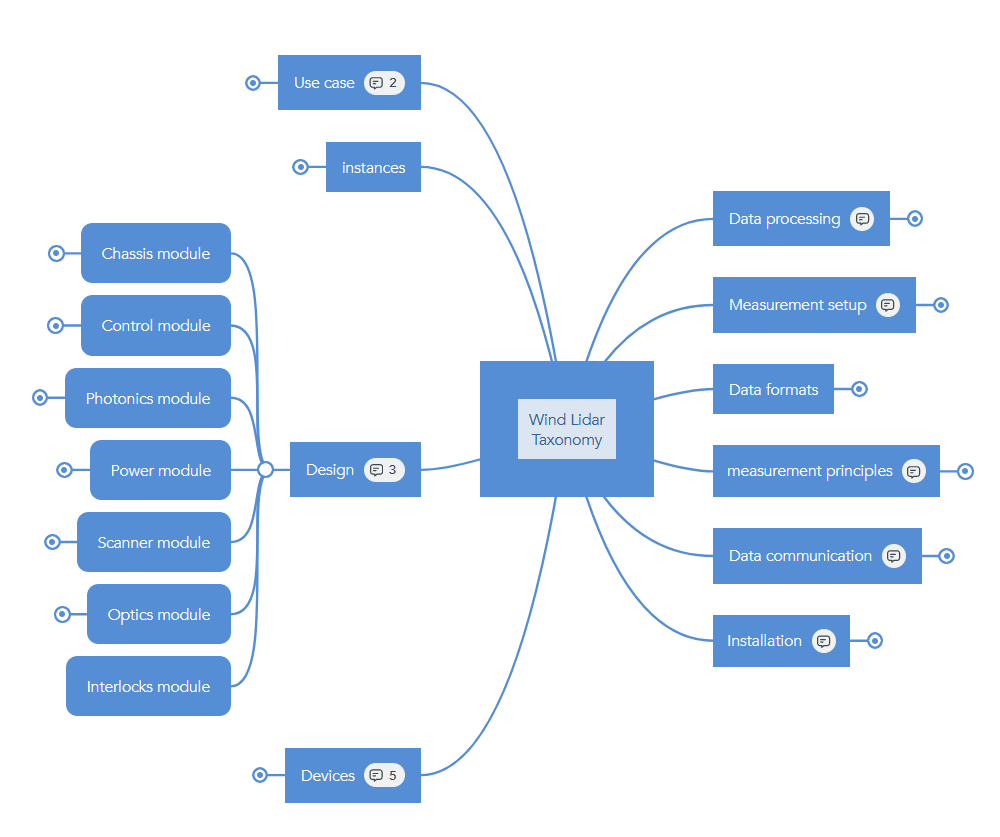
\includegraphics[width=12cm]{Figures/MindMap.PNG}
    \caption{The highest levels of the lidar taxonomy, from the broadest term ``wind lidar" to narrower terms. First and second hierarchical levels are shown, along with one third level which has been expanded.}
    \label{fig:tax}
\end{figure}
When the lidar concepts are endowed with extended information and their interrelationships specified, the lidar taxonomy is uplifted to a {\it lidar ontology}.

In addition, the lidar ontology is enhanced by the creation of a machine-readable data structure.
The wrappers sheet2rdf \cite{ref-Fiorelli2015} and Ontostack \cite{ref-OntoStack} have been used to orchestrate the framework necessary to deploy the lidar ontology. Their implementation is described in the following section.

\subsection{Implementation}
\label{subsec:implementation}
The ontology is deployed by means of a combination of several tools, brought together using GitHub Actions which enable automatic compilation and deployment. The workflow is as follows: 
\begin{description}
    
    \item [Input data sheet:] The input data sheet consists of a Google Sheets spreadsheet stored in Google Drive. The Google spreadsheet format eases the implementation of new data and its maintenance, compared to other more complex and less intuitive machine-readable formats like RDF. The spreadsheet has been populated with the lidar concepts and the related descriptive metadata considered to be most relevant for the wind lidar community. The source files for the wind lidar ontology and the spreadsheet are hosted in the repository  \textit{IEA-Wind-Task-32/wind-lidar-ontology} \cite{ref-IEA-Wind-Task-32-wind-lidar-ontology}.
    The Google spreadsheet format enables the ontology data to be read and manipulated by sheet2rdf in order for it to be converted to an RDF vocabulary, therefore to be handled as an online searchable asset. 
    
    \item [sheet2rdf:] The sheet2rdf framework builds on the excel2rdf \cite{ref-excel2rdf} workflow, enabling the acquisition and transformation of data sheets into RDF \cite{ref-sheet2rdf}. The specific sheet2rdf instance used in the present work is allocated in a GitHub repository \cite{ref-FAIRsheet2rdf} hosted by the FAIR Data Collective \cite{}. It contains the main functions that enable the conversion of the ontology information in the Google spreadsheet, into machine-actionable RDF format vocabulary, following SKOS standards. The sheet2rdf framework internally evaluates the quality of the SKOS concept scheme using qSKOS \cite{ref-W3C-qSKOS} and eventually deploys the RDF-formatted ontology to OntoStack. 
    
    sheet2rdf is a combination of software used to create a configurable automated process allocated as a GitHub Action workflow in \cite{ref-FAIRsheet2rdf}. Every time a user updates the excel sheet, the workflow can be manually triggered to update changes in the server.
    
    \item [OntoStack:] The Ontostack framework is a set of tools combined for the purpose of handling vocabularies and their RDF properties, as such yielded by sheet2rdf, and render them in human- and machine-readable formats, and as such, facilitates the deployment and visualisation of the wind lidar ontology.
    
    The lidar ontology is an instance of OntoStack and its online visualisation is hosted by the Wind and Energy Systems Department, at the Technical University  of Denmark (DTU).
    The wrapper OntoStack gathers functionalities from several tools enumerated here below \cite{ref-github-sheet2rdf}:
    \begin{itemize}
        \item Jena Fuseki \cite{ref-JenaFuseki}: a graph database based on SPARQL, a standard query language and protocol for linked open data on the web \cite{ref-SPARQL} that allows users to store and handle data in RDF format.
        \item Skosmos \cite{ref-Skosmos}:A web-based tool providing services for accessing controlled vocabularies.
        \item Tr\ae fik \cite{ref-Traefik}: An open-source edge router responsible for proper serving of URL requests 
    \end{itemize}
\end{description}

%\marginpar{[AC 20.12.22] I suggest splitting results and discussion into separate sections.}

\section{Results}
\label{sec:Results}

\subsection{Lidar ontology}

Structurally inspired by the OpenLidar Architecture \cite{}, this lidar ontology reports a dedicated list of concepts and definitions for supporting development of modular tools and processes for wind lidars. The selection and definition of the concepts included in the lidar ontology are the results of the joint effort and consensus of wind lidar experts, combining the information that describes the data and its associated metadata in a way that meets the needs and requirements of both academia and industry.

The consolidation of the ontology as it is nowadays took three main phases. The first step was to define the main structure of the ontology. This involved establishing the main nodes and relationships among them. First, second and third lidar ontology hierarchical levels are shown in Figure \ref{fig:tax}. Secondly, parent-child relationships among its 268 concepts were fully defined, as well as possible transitive relationships between tuples. Thirdly, lidar concepts were assigned according to authors' expertise to be elaborated and the results of their implementations were exposed, discussed and agreed upon by the members of the ontology group in recurrently scheduled meetings.

The ontology homepage contains information about the title of the ontology, a short description of the lidar ontology website and resource counts by type. Hosting for the online deployment is provided by the Technical University of Denmark (DTU) as an ontostack instance in the form of a look-up table. The human-friendly version of this interactive look-up table can be found at \cite{}.

\begin{table}[H] 
\caption{Information contained in each ontology concept. Due to its role and definition, ontology concepts might or might not contain all of the terms in the table.\label{Ontology_var}}
{\def\arraystretch{2}\tabcolsep=11pt
\begin{tabularx}{\textwidth}{lX}
\toprule
\toprule
\textbf{Variable}	\\
\midrule
\midrule
\textbf{Preferred term	}	& 	Name of the variable\\
\hline
\textbf{Definition}	& Consensual definition --- translated to several languages --- describing shortly the ontology concept and its role in the lidar field\\
\hline
\textbf{Broader/Narrower concept}	& If any, hierarchical relation and link to other broader/narrower terms within the ontology\\
\hline
\textbf{Entry terms}	& Alternative label\\
\hline
\textbf{Editorial note}	&  Some concepts contain editorial notes where  additional information is given \\
\hline
\textbf{In other languages}	& Preferred term in other languages\\
\hline
\textbf{URI}	& A Uniform Resource Identifier as a unique identifier of the physical resource\\
\hline
\textbf{Download this concept} & Machine-readable version of the ontology concept. Downloadable formats: RDF/XML, Turtle and JSON-LD\\
\bottomrule
\bottomrule
\end{tabularx}
}
% \noindent{\footnotesize{\textsuperscript{1} Due to its role and definition, ontology concepts might or might not contain all of the terms in the table}}
\end{table}

Users can explore the ontology and its content either alphabetically or hierarchically. The ontology's online version entries contain the fields included in Table \ref{Ontology_var}. Entry $Entry~terms$ contains information about the $alternative~label$ associated to a lidar asset. Each ontology concept has been unambiguously defined and labelled. The labelling has been aligned with the domain of knowledge (e.g. the $Velocity~azimuth~Display$ concept has been labelled as VAD, as it is commonly known within the lidar community) and the resulting $alternative~label$ can serve either for querying information within the framework or to be downloaded and integrated into digital workflows or codes. 

Queried information can be downloaded from the DTU server in three different formats, namely RDF/HTML, Turtle and Json, depending on user preferences. In the following subsection we present a python-based in-house method for downloading and coupling ontology terms to external digital workflows. 

% \begin{figure}[h]
%     \centering
%     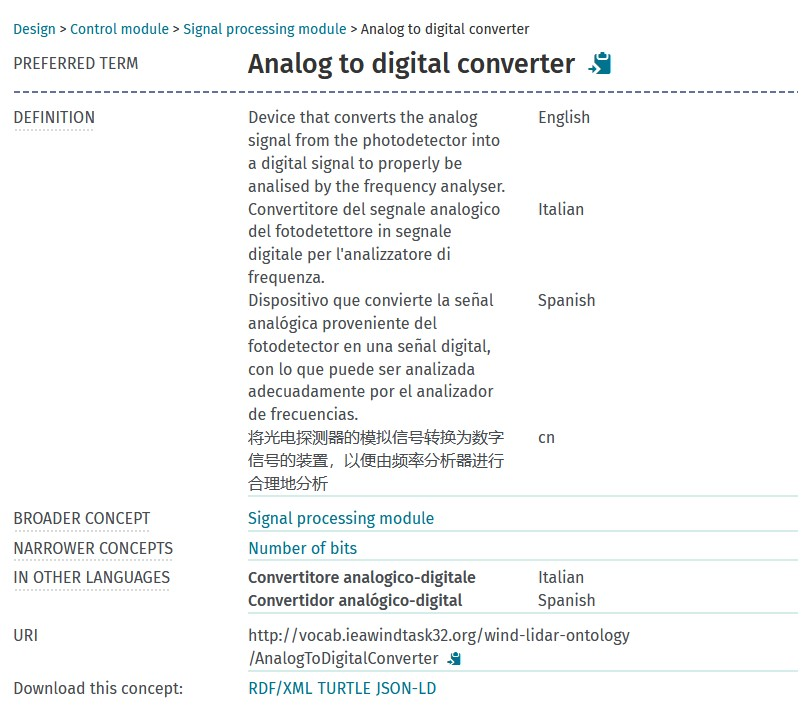
\includegraphics[width=9cm]{Figures/Concept.jpg}
    
%     \caption{First, second (Design) and third lidar taxonomy hierarchical levels.}
%     \label{tax}
% \end{figure}


% - How the ontology looks like 
% % - Process of how we get there
% - Talk about the concepts and the fields of each 
% - Output: RDF or Json
% - Conclusion of the definitions


\subsection{GitHub tool}
\label{GitTool}

In the Methodology section, we discussed the process how we established the wind lidar concepts and terminology based on the feedback from participants from different fields working in wind energy. During these discussions, we developed some tools to ease the application of metadata on datasets and allow standardisation across different application domains in wind energy. The Ontology tool is based on tools developed by the FAIR Data Collective discussed in the \ref{subsec:implementation}. The Ontology tool is available on github under the link: \href{https://github.com/PacoCosta/Extract-lidar-ontology-concepts}{https://github.com/PacoCosta/Extract-lidar-ontology-concepts} and we demonstrate an example using this tool here.

The general workflow for the demonstration is shown in Figure \ref{Ontology_workflow}.

\begin{figure}[h!]
    \centering
    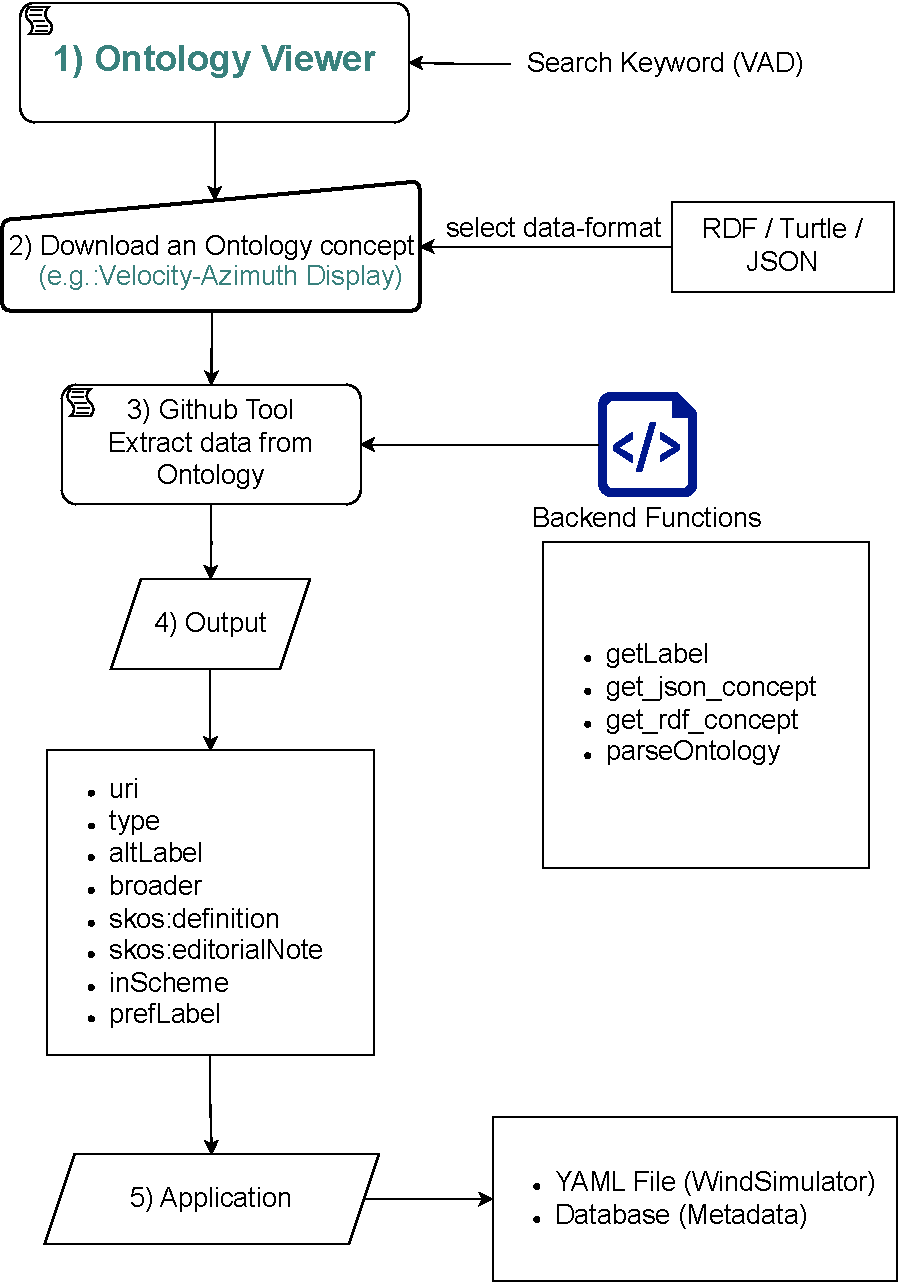
\includegraphics[width=\textwidth]{Figures/Ontology_flow.drawio.pdf}
    \caption{General workflow for Ontology concepts}
    \label{Ontology_workflow}
\end{figure}

The workflow is divided into the following elements:

\begin{enumerate}
    \item Search the Ontology database for a keyword (e.g. VAD).
    \item Download the concept in form of RDF, Turtle or JSON file format.
    \item Select the language, extract the concept into python or any other language from above-mentioned file formats.
    \item Apply the output (metadata parameters e.g. definition, preferred Label, uri, etc.) to your application
\end{enumerate}

The \textit{Ontology Viewer} is a webserver where the definitions are stored and is hosted by DTU. The block \textit{Download an Ontology concept} refers to a user action of searching a keyword, selecting the definition and downloading this definition from the Ontology Viewer. The block \textit{Github Tool} refers to the python tool developed to extract data from the downloaded definition and making it available for further use. The block \textit{Backed Functions} refers to the python routines that help the user in fetching definitions and finally the block \textit{Output} refers to the metadata definitions output.

In order to merge the Ontology with any application, there are two alternatives. In the first option, one can download specific keywords from the webserver based Ontology database in fileformats like RDF, Turtle or JSON. In the second option, a database file already existing in the Github tool can be accessed and filtered through any programming tool (e.g. Python) for specific keywords. The steps 1,2,3,4 can be set accordingly in the latter case. We describe the first step in detail here, as this is more exhaustive and provides a better overview of the steps involved.

The downloaded definition file format is then read using the Github tool as referred earlier. Using the code snippets shown in the next sections, the data is fetched from the Ontology files in specific language (e.g. English). The output from the fetched data refers to the metadata parameters that describe the definition of the Ontology variable which include uri, type, alternative and preferred labels, definitions and editorial notes.

\begin{tcolorbox}
    Workflow block 2: Fetch the concept from downloaded file format
\begin{python}
# Open the file that users download from 
#  (https://data.windenergy.dtu.dk/ontologies/view/ontolidar/en/)
with open(r'.\Ontology_Concepts\VAD_da', encoding='utf-8') as f:
    d = json.load(f)

print(d)
\end{python}
\end{tcolorbox}

\begin{tcolorbox}
    Workflow block 3: Using the Github tool, setting input parameters
\begin{python}
#Getting definition of the concept
from fun.getLabel import getLabel
path = r'./Ontology_Concepts/VAD_da'
Alternative_Label = getLabel(path, key = "altLabel", lang='en', index_inScheme=1)

# get individual key value pairs depending on the key requested
Definition = getLabel(path, key="skos:definition", lang='en', index_inScheme=1)
Preferred_Label = getLabel(path, key="prefLabel", lang='en', index_inScheme=1)
Alternative_Label = getLabel(path, key = "altLabel", lang='en', index_inScheme=1)

#Save in a new dictionary
Lidar_Dictionary['Definition']=Definition
Lidar_Dictionary['Preferred Label']=Preferred_Label
Lidar_Dictionary['Alternative Label']=Alternative_Label
print(Definition)
\end{python}
\end{tcolorbox}

\begin{tcolorbox}
    Workflow block 3: using the Github tool
    \begin{python}
    # import the whole concept with main variables from json file
    path = r'../Ontology_Concepts/VAD_da'
    lang = "en"
    concept_json = get_json_concept(path, lang)

    # import the whole concept with main variables from turtle file
    path = r'../Ontology_Concepts/vad.ttl'
    lang = "en"
    fmt = 'ttl'
    concept_rdf = get_rdf_concept(path, lang, fmt)
\end{python}
\end{tcolorbox}

\begin{tcolorbox}
    Workflow block 4: Output from the Github tool
    \begin{python}
    {   'altLabel': 'VAD',
    'broader': {   'uri': 'http://vocab.ieawindtask32.org/wind-lidar-ontology/WindfieldReconstruction'},
    'inScheme': {'uri': 'http://vocab.ieawindtask32.org/wind-lidar-ontology/'},
    'prefLabel': 'Velocity-azimuth display',
    'skos:definition': 'VAD is a method of analyzing data from a complete '
                       'conical scan whereby many closely spaced azimuthal '
                       'points may be sampled by the lidar, and the data are '
                       'used to estimate the wind speed at each height using a '
                       'statistical fitting method.',
    'skos:editorialNote': 'The VAD method is described in Lhermitte (1966) and '
                          'Browning and Wexler (1968).',
    'type': 'skos:Concept',
    'uri': 'http://vocab.ieawindtask32.org/wind-lidar-ontology/VelocityAzimuthDisplay'}
\end{python}
\end{tcolorbox}

\begin{tcolorbox}
    Workflow block 5: Concept and parameters in the YAML file
    \begin{python}

# Edit local yaml file
from fun.edit_yaml_from_ontology import edit
edit(local_yaml,tag,fields2change,Lidar_Dictionary) 

'''
# Find the concept and parameters within the local
# yaml file (dictionary like) 

def find(obj,tag):
    
    # Function digging into the (likely nested) python dictionary to find the targeted concept and field to be changed.
    
    if tag in obj:
        yield obj[tag]
    for k,v in obj.items():       
        if isinstance(v,dict):
            for i in find(v,tag):
                yield i                

# Open/close, edit and save the local yaml file with the updated info     

def edit(local_yaml,tag,fields2change,Lidar_Dictionary):
    import ruamel.yaml
    yaml = ruamel.yaml.YAML()
    
    # Read local yaml file and update the desired fields with the info from 
    # the downloaded concept  
    with open (local_yaml,"r") as file:
        data = yaml.load_all(file)
        for obj in data:
            for val in find(obj,tag):
                for i in fields2change:
                    if not val[i]:
                        val[i]=Lidar_Dictionary[i]
    
    # Edit the desired fields of the local file
    with open(local_yaml, "w") as file:
        yaml.dump(obj, file)
'''    
\end{python}
\end{tcolorbox}


(...) In a last step, a local yaml file, used as an input file for a lidar simulator, is updated with info from the ontology. By selecting the fields we want to edit, the info from the ontology is incorporated into the local file. The local variable/concept will be aligned with the ontology concept through its \texttt{Alternative Label}. The function  \texttt{edit\_yaml\_from\_ontology.edit}:

\begin{enumerate}
    \item reads user's lidar input yaml local template and converts it into a python dictionary,
    \item finds, within the nested dictionary, concepts and fields aimed to be changed. Concept and targeted fields are introduced by the user. These are contained in the variable \texttt{fields2change}
    \item updates the fields in the local template with information extracted from the downloaded ontology concept and saves the changes. The updating process preserves information contained in the local yaml file. 
    
\end{enumerate} 




\subsection{Benefits and limitations}
The lidar ontology provides many benefits to the lidar community.
The lidar ontology provides standardisation of terminology within the lidar knowledge domain, and re-use of the domain knowledge with the minimum of ambiguity.
The lidar ontology is a versatile framework which has the adaptability to incorporate new concepts and developments within the lidar industry.
It is anticipated that the lidar ontology will be widely used within both the lidar industry and the wider wind industry.
The open-source framework will promote sharing of the lidar ontology and increase the possibility of collaboration through modification and enhancement of concepts and terminology. 
The concepts and terminology to date have been established based on common usage within the industry over several decades.
The lidar ontology framework has been developed to maximise accessibility through the use of well established standard data structures such as RDF and the gitHub software platform.

Despite these recognised benefits, possible limitations of the lidar ontology should also be acknowledged.
The software framework may represent a barrier to those users with less experience, and may prove to be difficult to integrate into existing software structures.
Several ontologies exist within the wind energy industry and there exists the possibility that conflicts may arise in the terminology.
A technological framework such as an ontology requires ownership and maintenance, which requires ongoing commitment to the project.
This requires a level of funding and time resource dedicated to the lidar ontology project. 

% \subsection{Examples}
% Examples

% \subsubsection{Transfer data, tools, and knowledge Open library}
% Example

% \subsubsection{Standardize input files}
% Example

% \subsection{Benefits and limitations}
% Benefits and limitations

\section{Discussion}
\label{sec:Discussion}
This article has given an overview of the development of the lidar ontology, which has been developed with the aim of establishing an industry-wide consensus on wind lidar concepts and terminology.

The lidar ontology was developed by garnering opinions from several parties within the wind energy and lidar industry and academic research groups on the relevant subject matter, and subsequent incorporation into an ontology framework. 
An initial ontology structure was proposed and, subsequently, through a series of meetings, a consensus was reached on what should constitute the final concept definitions and terminology.
A diverse range of viewpoints has ensured that a wide range of concepts and definitions has been captured within the ontology. 
The lidar ontology contains more than 200 terms and concepts with definitions, and alternative names where appropriate. In addition, each term definition is given in four languages. 
The ontology has been made available in RDF data format, which provides a convenient framework to model a controlled vocabulary and define properties, relationships, constraints and axioms among its concepts.
It is anticipated that the lidar community and industry will benefit from the lidar ontology.


% Issues and challenges?

% ----------
% Opportunities and Challenges
% ----------
% [AC 20.12.22] introduced new section to replace / capture material from conclusions


\section{Outlook}
\label{sec:Outlook}
% Carlo and Andy
    % 1. Keep ontology up to date
    % 2. Combine with exitisting wind community ontologies (TASK37)
Things to consider: Engagement with industry; User participation and user feedback; Future updates of the ontology, published versions; Workshops?

\section{Acknowledgments}
All participants, collectives and institutions that do not appear in the list of authors.


%%%%%%%%%%%%%%%%%%%%%%%%%%%%%%%%%%%%%%%%%%
\vspace{6pt} 

%%%%%%%%%%%%%%%%%%%%%%%%%%%%%%%%%%%%%%%%%%
%% optional
%\supplementary{The following supporting information can be downloaded at:  \linksupplementary{s1}, Figure S1: title; Table S1: title; Video S1: title.}

% Only for the journal Methods and Protocols:
% If you wish to submit a video article, please do so with any other supplementary material.
% \supplementary{The following supporting information can be downloaded at: \linksupplementary{s1}, Figure S1: title; Table S1: title; Video S1: title. A supporting video article is available at doi: link.}

%%%%%%%%%%%%%%%%%%%%%%%%%%%%%%%%%%%%%%%%%%
\authorcontributions{For research articles with several authors, a short paragraph specifying their individual contributions must be provided. The following statements should be used ``Conceptualization, X.X. and Y.Y.; methodology, X.X.; software, X.X.; validation, X.X., Y.Y. and Z.Z.; formal analysis, X.X.; investigation, X.X.; resources, X.X.; data curation, X.X.; writing---original draft preparation, X.X.; writing---review and editing, X.X.; visualization, X.X.; supervision, X.X.; project administration, X.X.; funding acquisition, Y.Y. All authors have read and agreed to the published version of the manuscript.'', please turn to the  \href{http://img.mdpi.org/data/contributor-role-instruction.pdf}{CRediT taxonomy} for the term explanation. Authorship must be limited to those who have contributed substantially to the work~reported.}

\funding{Please add: ``This research received no external funding'' or ``This research was funded by NAME OF FUNDER grant number XXX.'' and  and ``The APC was funded by XXX''. Check carefully that the details given are accurate and use the standard spelling of funding agency names at \url{https://search.crossref.org/funding}, any errors may affect your future funding.}

\institutionalreview{In this section, you should add the Institutional Review Board Statement and approval number, if relevant to your study. You might choose to exclude this statement if the study did not require ethical approval. Please note that the Editorial Office might ask you for further information. Please add “The study was conducted in accordance with the Declaration of Helsinki, and approved by the Institutional Review Board (or Ethics Committee) of NAME OF INSTITUTE (protocol code XXX and date of approval).” for studies involving humans. OR “The animal study protocol was approved by the Institutional Review Board (or Ethics Committee) of NAME OF INSTITUTE (protocol code XXX and date of approval).” for studies involving animals. OR “Ethical review and approval were waived for this study due to REASON (please provide a detailed justification).” OR “Not applicable” for studies not involving humans or animals.}

\informedconsent{Any research article describing a study involving humans should contain this statement. Please add ``Informed consent was obtained from all subjects involved in the study.'' OR ``Patient consent was waived due to REASON (please provide a detailed justification).'' OR ``Not applicable'' for studies not involving humans. You might also choose to exclude this statement if the study did not involve humans.

Written informed consent for publication must be obtained from participating patients who can be identified (including by the patients themselves). Please state ``Written informed consent has been obtained from the patient(s) to publish this paper'' if applicable.}


\dataavailability{The Lidar ontology viewer is available on:  \href{https://data.windenergy.dtu.dk/ontologies/view/ontolidar/en/}{Lidar ontology viewer}. The GitHub tool is available on github under: \href{https://github.com/PacoCosta/Extract-lidar-ontology-concepts}{GitHub tool}.} 
% \dataavailability{In this section, please provide details regarding where data supporting reported results can be found, including links to publicly archived datasets analyzed or generated during the study. Please refer to suggested Data Availability Statements in section ``MDPI Research Data Policies'' at \url{https://www.mdpi.com/ethics}. If the study did not report any data, you might add ``Not applicable'' here.} 

\acknowledgments{In this section you can acknowledge any support given which is not covered by the author contribution or funding sections. This may include administrative and technical support, or donations in kind (e.g., materials used for experiments).}

\conflictsofinterest{The authors declare no conflict of interest. The founders had no role in the design of the study; in the collection, analyses, or interpretation of data; in the writing of the manuscript; or in the decision to publish the~results.}


% Authors must identify and declare any personal circumstances or interest that may be perceived as inappropriately influencing the representation or interpretation of reported research results. Any role of the funders in the design of the study; in the collection, analyses or interpretation of data; in the writing of the manuscript; or in the decision to publish the results must be declared in this section. If there is no role, please state ``The funders had no role in the design of the study; in the collection, analyses, or interpretation of data; in the writing of the manuscript; or in the decision to publish the~results''.} 

%%%%%%%%%%%%%%%%%%%%%%%%%%%%%%%%%%%%%%%%%%
%% Optional
\sampleavailability{Samples of the compounds ... are available from the authors.}

%% Only for journal Encyclopedia
%\entrylink{The Link to this entry published on the encyclopedia platform.}

\abbreviations{Abbreviations}{
The following abbreviations are used in this manuscript:\\

\noindent 
\begin{tabular}{@{}ll}
Lidar & Light Detection And Ranging\\
OEM & Original Equipment Manufacturer\\
FAIR & Findable, Accessible, Interoperable and Reusable\\
RDF & Resource Description Framework\\
SKOS & Simple Knowledge Organisation System
\end{tabular}
}

%%%%%%%%%%%%%%%%%%%%%%%%%%%%%%%%%%%%%%%%%%

%%%%%%%%%%%%%%%%%%%%%%%%%%%%%%%%%%%%%%%%%%
\begin{adjustwidth}{-\extralength}{0cm}
%\printendnotes[custom] % Un-comment to print a list of endnotes

\reftitle{References}

% Please provide either the correct journal abbreviation (e.g. according to the “List of Title Word Abbreviations” http://www.issn.org/services/online-services/access-to-the-ltwa/) or the full name of the journal.
% Citations and References in Supplementary files are permitted provided that they also appear in the reference list here. 

%=====================================
% References, variant A: external bibliography
%=====================================
%\bibliography{your_external_BibTeX_file}
\bibliography{references}

%=====================================
% References, variant B: internal bibliography
%=====================================
% \begin{thebibliography}{999}

% \bibitem[Author1(year)]{ref-Liu}
% Liu, Z.;Barlow, J. F.;Chan, P.;Fung, J. C. H.;Li, Y.;Ren, C.;Mak, H. W. L.;Ng, E., A Review of Progress and Applications of Pulsed Doppler Wind LiDARs. {\em Remote Sensing} {\bf 2019}, {\em 11}, 2522.

% \end{thebibliography}


% If authors have biography, please use the format below
%\section*{Short Biography of Authors}
%\bio
%{\raisebox{-0.35cm}{\includegraphics[width=3.5cm,height=5.3cm,clip,keepaspectratio]{Definitions/author1.pdf}}}
%{\textbf{Firstname Lastname} Biography of first author}
%
%\bio
%{\raisebox{-0.35cm}{\includegraphics[width=3.5cm,height=5.3cm,clip,keepaspectratio]{Definitions/author2.jpg}}}
%{\textbf{Firstname Lastname} Biography of second author}

% For the MDPI journals use author-date citation, please follow the formatting guidelines on http://www.mdpi.com/authors/references
% To cite two works by the same author: \citeauthor{ref-journal-1a} (\citeyear{ref-journal-1a}, \citeyear{ref-journal-1b}). This produces: Whittaker (1967, 1975)
% To cite two works by the same author with specific pages: \citeauthor{ref-journal-3a} (\citeyear{ref-journal-3a}, p. 328; \citeyear{ref-journal-3b}, p.475). This produces: Wong (1999, p. 328; 2000, p. 475)

%%%%%%%%%%%%%%%%%%%%%%%%%%%%%%%%%%%%%%%%%%
%% for journal Sci
%\reviewreports{\\
%Reviewer 1 comments and authors’ response\\
%Reviewer 2 comments and authors’ response\\
%Reviewer 3 comments and authors’ response
%}
%%%%%%%%%%%%%%%%%%%%%%%%%%%%%%%%%%%%%%%%%%
\end{adjustwidth}
\end{document}

